\documentclass[border=10pt]{standalone}
\usepackage[utf8]{inputenc}
\usepackage[T1]{fontenc}
\usepackage{tikz}
\usepackage{circuitikz}
\usetikzlibrary{shapes.geometric}
\usetikzlibrary{arrows}

% Farbdefinitionen
\colorlet{arrowColor}{gray!40}
\colorlet{componentFill}{gray!15}
\colorlet{highlightRed}{red}
\colorlet{highlightBlue}{blue} % Geändert von Grün zu Blau

\begin{document}

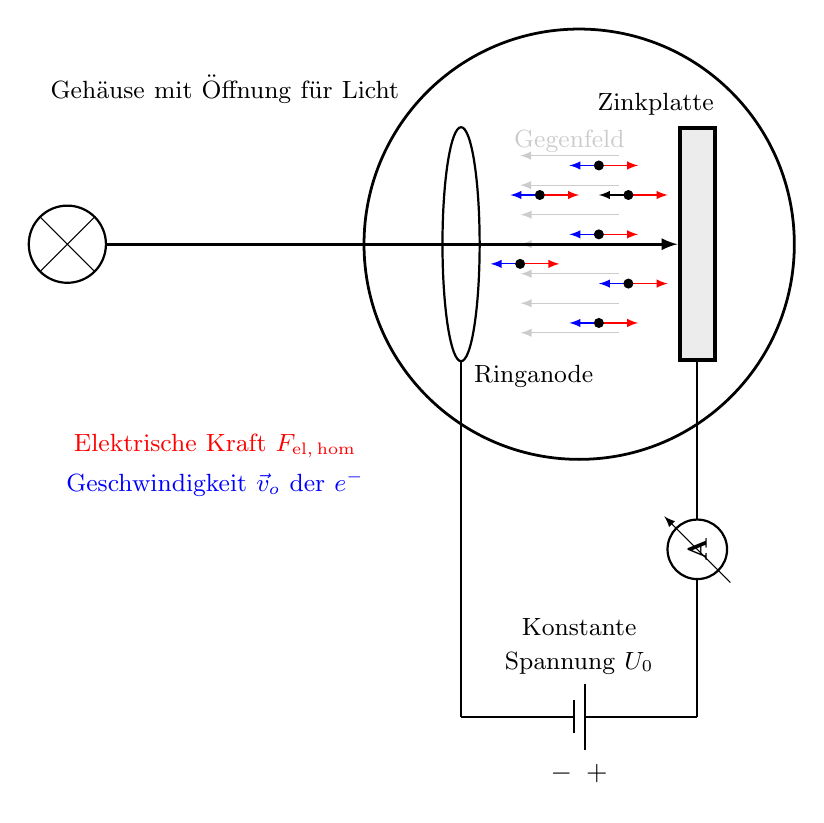
\begin{tikzpicture}
	% --- Feldlinien (grau, zeigen nach links) ---
	\draw[-latex] (8.125, 5.125) -- (7.75, 5.125);
	\path[draw=arrowColor, -latex] (8.006, 3.75) -- (6.756, 3.75);
	\path[draw=arrowColor, -latex] (8, 5.625) -- (6.75, 5.625);
	\path[draw=arrowColor, -latex] (8.006, 4.875) -- (6.756, 4.875);
	\path[draw=arrowColor, -latex] (8.006, 4.5) -- (6.756, 4.5);
	\path[draw=arrowColor, -latex] (8.006, 3.375) -- (6.756, 3.375);
	\path[draw=arrowColor, -latex] (8, 5.25) -- (6.75, 5.25);
	\path[draw=arrowColor, -latex] (8.006, 4.125) -- (6.756, 4.125);

    % --- Lichtstrahl (dick, 1pt) ---
	\draw[-latex, line width=1pt] (1.5, 4.5) -- (8.75, 4.5);

    % --- Schaltungskomponenten ---
	\draw (9, 0.25) to[ammeter] (9, 1);
	\draw (7.625, -1.5) to[battery1, l={$-\enspace+$}] (7.375, -1.5);
	\draw[line width=0.8pt] (9, 0.25) -- (9, -1.5);
	\draw[line width=0.8pt] (9, 1) -| (9, 3);
	\draw[line width=0.8pt] (6, 3) -- (6, -1.5);
	\draw[line width=0.8pt] (9, -1.5) -- (7.564, -1.5);
	\draw[line width=0.8pt] (7.425, -1.5) |- (6, -1.5);

    % --- Geometrische Formen ---
	\node[shape=rectangle, fill=componentFill, draw, line width=1.5pt, minimum width=0.447cm, minimum height=2.947cm] at (9, 4.5){};
	\node[shape=ellipse, draw, line width=0.8pt, minimum width=0.472cm, minimum height=2.972cm] at (6, 4.5){};
	\node[mixer] at (1, 4.5){};
    \node[shape=circle, draw, line width=1pt, minimum width=5.465cm] at (7.5, 4.5){};

    % --- Geschwindigkeitsvektoren (BLAU, zeigen nach links) ---
	\draw[-latex, color=highlightBlue] (6.75, 4.25) -- (6.375, 4.25);
	\draw[-latex, color=highlightBlue] (7.75, 3.5) -- (7.375, 3.5);
	\draw[-latex, color=highlightBlue] (8.125, 4) -- (7.75, 4);
	\draw[-latex, color=highlightBlue] (7, 5.125) -- (6.625, 5.125);
	\draw[-latex, color=highlightBlue] (7.75, 5.5) -- (7.375, 5.5);
	\draw[-latex, color=highlightBlue] (7.75, 4.625) -- (7.375, 4.625);

    % --- Kraftvektoren (ROT, zeigen nach rechts) ---
	\draw[-latex, color=highlightRed] (7.75, 5.5) -- (8.25, 5.5);
	\draw[-latex, color=highlightRed] (8.125, 5.125) -- (8.625, 5.125);
	\draw[-latex, color=highlightRed] (7.75, 4.625) -- (8.25, 4.625);
	\draw[-latex, color=highlightRed] (6.75, 4.25) -- (7.25, 4.25);
	\draw[-latex, color=highlightRed] (7.75, 3.5) -- (8.25, 3.5);
	\draw[-latex, color=highlightRed] (8.125, 4) -- (8.625, 4);
    \draw[-latex, color=highlightRed] (7, 5.125) -- (7.5, 5.125);

    % --- Beschriftungen ---
	\node[shape=rectangle, minimum width=1.59cm, minimum height=0.465cm] at (7.375, 5.875){} 
        node[anchor=south, align=center, text width=1.554cm, inner sep=1pt] at (7.375, 5.625){\textcolor{arrowColor}{\small Gegenfeld}};

	\node[shape=rectangle, minimum width=4.715cm, minimum height=0.465cm] at (3, 6.5){} 
        node[anchor=south, align=center, text width=4.679cm, inner sep=1pt] at (3, 6.25){\small Gehäuse mit Öffnung für Licht};

	\node[shape=rectangle, minimum width=1.59cm, minimum height=0.465cm] at (8.438, 6.275){} 
        node[anchor=south east, align=right, text width=1.554cm, inner sep=1pt] at (9.25, 6.1){\small Zinkplatte};

	\node[shape=rectangle, minimum width=1.59cm, minimum height=0.465cm] at (6.938, 2.75){} 
        node[anchor=north west, align=left, text width=1.554cm, inner sep=1pt] at (6.125, 3){\small Ringanode};

	\node[shape=rectangle, minimum width=2.027cm, minimum height=0.465cm] at (7.5, -0.75){} 
        node[anchor=south, align=center, text width=1.992cm, inner sep=1pt] at (7.5, -1){\small Konstante Spannung $U_0$};

	\node[shape=rectangle, minimum width=4.715cm, minimum height=0.465cm] at (2.875, 2){} 
        node[anchor=south, align=center, text width=4.679cm, inner sep=1pt] at (2.875, 1.75){\textcolor{highlightRed}{\small Elektrische Kraft $F_\mathrm{el,\,hom}$}};
        
    % Legende für Geschwindigkeit jetzt BLAU (highlightBlue)
	\node[shape=rectangle, minimum width=4.715cm, minimum height=0.465cm] at (2.875, 1.5){} 
        node[anchor=south, align=center, text width=4.679cm, inner sep=1pt] at (2.875, 1.25){\textcolor{highlightBlue}{\small Geschwindigkeit $\vec{v}_o$ der $e^-$}};

    % --- Elektronen (Nodes) in den Vordergrund verschoben ---
    % Durch das Zeichnen am Ende liegen sie über den Vektorpfeilen
	\node[circ] at (7.75, 3.5){};
	\node[circ] at (7, 5.125){};
	\node[circ] at (6.75, 4.25){};
	\node[circ] at (8.125, 4){};
	\node[circ] at (8.125, 5.125){};
	\node[circ] at (7.75, 4.625){};
	\node[circ] at (7.75, 5.5){};

\end{tikzpicture}

\end{document}